% Chapter Template

\chapter{Timeouts} % Main chapter title

\label{Chapter5} % Change X to a consecutive number; for referencing this chapter elsewhere, use \ref{ChapterX}

In this chapter, the two timeout strategies developed for this project are explained.\\\\
As previously said in this document, some users may need a result before a specific time. When timeouts are used, the solution to the problem may not be the optimal one, as explained in the following lines.

\section{Simple timeout}
For this strategy, the user defines a maximum number of seconds that each call to the sat-solver can take. In other words, the amount of time that a value between \emph{min} and \emph{max} is checked to be the optimal or not. \\\\
To accomplish this behaviour, a new thread is created, and the call to the sat-solver is executed in parallel while the main thread looks that the elapsed time is less than the timeout defined by the user.  \\\\
When the elapsed time is longer than the time defined by the user, the main thread kills the sat-solver execution and assumes that the problem was \emph{unsatisfiable}. This assumption leads to suboptimal solutions but correct solutions. However, if the assumption were that the problem was \emph{satisfiable}, then this could point to wrong solutions. \\\\
For example:
\subsection{Linear search}
\begin{center}
	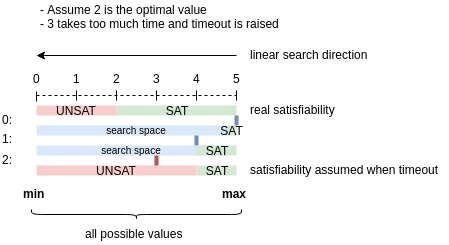
\includegraphics[width=0.8\textwidth]{Figures/SimpleTimeoutLinearSearch.png}
	\captionof{figure}{Simple timeout with linear search}
	\label{SimpleTimeoutLinearSearch}
\end{center}
As the reader can see in the figure above\ref{SimpleTimeoutLinearSearch}, there is a Pseudo-Boolean minimisation problem which its minimum value is 2, and the cost function values go from 0 to 5. Because it is using \emph{Linear search} algorithm, it will start from 5 and will descend until the problem is \emph{unsatisfiable} or 0.\\
If 2 is the minimum value, it means that below 2 all is \emph{unsatisfiable} and from all values greater equal than 2 are \emph{satisfiable}. We also assume that the call to the sat-solver when trying 3 will take longer than the time defined by the user, i.e. a timeout will be raised. \\\\
At the first iteration of the algorithm, \emph{0:}, the CNF Pseudo-Boolean constraints AND $cost function \leq 5$ will be generated which will return SAT.\\
At the second iteration, \emph{1:}, the CNF Pseudo-Boolean constraints AND $cost function \leq 4$ will be generated, and this also will return SAT.\\
At the third iteration, \emph{2:}, the CNF Pseudo-Boolean constraints AND $cost function \leq 3$ will be generated. We know that this should return satisfiable but because it takes too long, the timeout is raised, and unsatisfiable is returned. The algorithm assumes that all the values below 3 will also be unsatisfiable and ends the search. 4 was the last satisfiable value found, so it is returned as the minimum value. \\\\
As the reader can see, this is not the optimal solution but a correct one.

\subsection{Binary search}
\begin{center}
	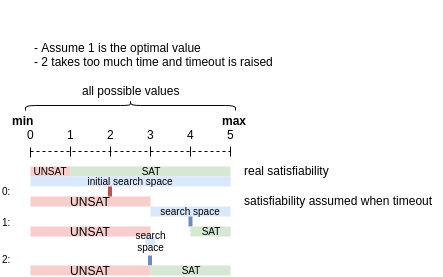
\includegraphics[width=0.8\textwidth]{Figures/SimpleTimeoutBinarySearch.png}
	\captionof{figure}{Simple timeout with binary search}
	\label{SimpleTimeoutBinarySearch}
\end{center}
In this case, the search algorithm used is \emph{Binary search}. We assume a Pseudo-Boolean minimisation problem where the minimum value is 1, the values of the cost function are between 0 ad 5, and that the call to the sat-solver when trying 2 will take longer than the time defined by the user, i.e. a timeout will be raised.\\\\
At the first iteration, \emph{0:}, the search space is between 0 and 5, and the algorithm knows nothing about the satisfiability of the problem. 2 is the middle value so the CNF Pseudo-Boolean constraints AND $cost function \leq 2$ is generated. Because of the problem definition, this is satisfiable, but it takes longer than the time defined by the user and the timeout is raised.\\
The execution of the sat-solver is stopped, and it assumes the CNF is unsatisfiable.\\\\
At this point, it assumes that 2 and all the values under it are unsatisfiable and the search space is reduced to 3 to 5.\\
Iterations 1, 2 proceed as a regular Binary search execution, and finally, the value 3 is returned as the optimal one.\\\\
As before, the given solution is not optimal but correct.

\section{General timeout}
For this strategy, the user defines a maximum number of seconds that the whole problem can take. In other words, the amount of time that the user will wait for an answer. \\\\
To accomplish this behaviour, a new thread is created, and the call to the search algorithm is executed in parallel while the main thread looks that the elapsed time is less than the timeout defined by the user.  \\\\
When the elapsed time is longer than the time defined by the user, the main thread kills the search algorithm execution and assumes that it finished normally, i.e. the last value found is returned as the minimum one. This assumption leads to suboptimal solutions but correct solutions. However, if the assumption were that the problem was satisfiable, then this could point to wrong solutions. 
\subsection{Linear search}
\begin{center}
	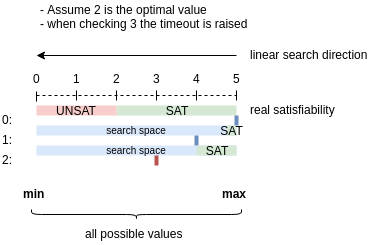
\includegraphics[width=0.8\textwidth]{Figures/GeneralTimeoutLinearSearch.png}
	\captionof{figure}{General timeout with linear search}
	\label{GeneralTimeoutLinearSearch}
\end{center}
As the reader can see in the figure above\ref{GeneralTimeoutLinearSearch}, there is a Pseudo-Boolean minimisation problem which its minimum value is 2, and the cost function values go from 0 to 5. Because it is using Linear search algorithm, it will start from 5 and will descend until the problem is unsatisfiable or 0. \\
If 2 is the minimum value, it means that below 2 all is unsatisfiable and from all values greater equal than 2 are satisfiable.  We also assume that when trying 3 will take longer than the time defined by the user, i.e. a timeout will be raised.\\\\
At the first iteration of the algorithm, \emph{0:}, the CNF Pseudo-Boolean constraints AND $cost function \leq 5$ will be generated which will return SAT.\\
At the second iteration, \emph{1:}, the CNF Pseudo-Boolean constraints AND $cost function \leq 4$ will be generated, and this also will return SAT.\\
At the third iteration, \emph{2:}, the CNF Pseudo-Boolean constraints AND $cost function \leq 3$ will be generated. Then the timeout is raised, and the last satisfiable value found, 4, is returned as the minimum one.\\\\
As the reader can see, this is not the optimal solution but a correct one. 

\subsection{Binary search}
\begin{center}
	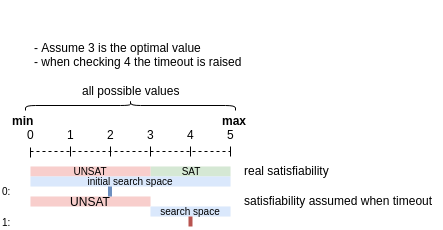
\includegraphics[width=0.8\textwidth]{Figures/GeneralTimeoutBinarySearch.png}
	\captionof{figure}{General timeout with binary search}
	\label{GeneralTimeoutBinarySearch}
\end{center}
In this case, the search algorithm used is Binary search. We assume a Pseudo-Boolean minimisation problem where the minimum value is 3, the values of the cost function are between 0 and 5, and that when trying 4 the timeout will be raised. \\\\
At the first iteration, \emph{0:}, the search space is between 0 and 5, and the algorithm knows nothing about the satisfiability of the problem. 2 is the middle value so the CNF Pseudo-Boolean constraints AND $cost function \leq 2$ is generated. Because 2 is unsatisfiable, the search space is reduced to 3 to 5, and the next value to be checked is 4. \\\\
When checking 4, the timeout is raised, and the search space becomes empty. Because there are no more elements to be checked, the last minimum value found is returned, which in this case there is not one, i.e. the software returns unsatisfiable. \\\\
Like before, the given solution is not optimal but correct. 